% better title
\chapter{Graph and Rules}
% nog niet goed

First, a theorethical model is defined. This model allows us to illustrate the information, problems and respective solutions concerning our challenge to disambiguate people around the web. We introduce a three-layer graph model that will integrate structural, informational and algorithmic aspects while respecting the foundation acknowledgements we established earlier (REF). In the next chapter, we show how this model can be practically realised.

\section{Graph as a model}

\begin{mydef}
A \textbf{Fact} is a certainty derived from a piece of information.
\end{mydef}

\begin{mydef}
A \textbf{Discovery} is a fact that proofs the existence of a certain entity (an address, a publication, \ldots)
\end{mydef}

\begin{mydef}
A \textbf{Relation} is a fact that denotes a relation between two entities \ldots
\end{mydef}

\section{Three layer model: structural layer}

% introductie

\subsection{Instances and Authors}

% welke decision, definieer!
One of the main responsibilities of the structural layer is reflecting a decision through a change in structure. It is clear that this is very important. Deciding which physical author some information belongs to is the main issue of our thesis. This part focusses on how the model adapt to such a decision. We first explain the first solution that would probably come to mind and the shortcoming of it. Then we provide a solution that deals with these shortcomings.

\paragraph{Merging} Assume that we have a source of information that has two occurences of the same name X. Along each of these occurrences, we find some extra information on the person(s) with this name. At first we do not know if this is just one person or two persons who share the same name. Now suppose that we have an algorithm that claims the latter. Therefore we have made a decision that the two pieces of information depict the same actual person. The idea is now to simply merge these two chunks of information, representing exactly one person. The situation together with its outcome is illustrated in \autoref{clusteringsimple}.

The main problem with this solution is that it does not take all of the foundation acknowledgements into account. Merging two authors is a definitive operation, it can not be undone. We operate in a very dynamic environment, our system is subject to constant change. Therefore it is wise to not base a decision only on past information. Future information can provide new motives to make another decision.

\begin{figure}[htbp]
	\centering
		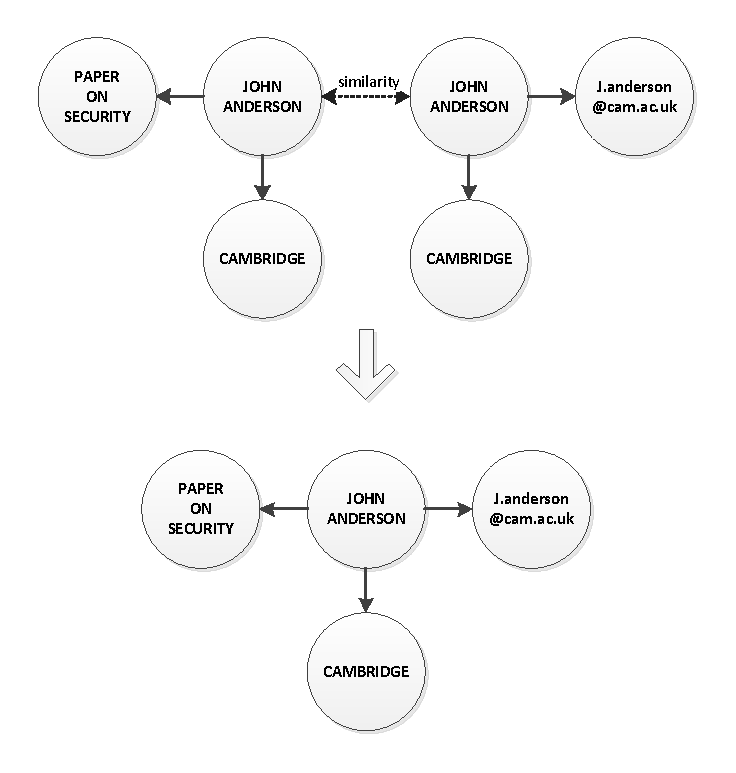
\includegraphics[width=0.6\textwidth]{fig/clusteringsimple}
	\caption{Merging of two authors}
	\label{fig:clusteringsimple}
\end{figure}

\paragraph{Grouping} To solve this problem, we define a new concept: instances. An author is no longer defined by an author node and its property nodes. Instead, an extra level is added: an actual author is now equivalent with a collection of instances. Let us first formally define instances:

\begin{mydef}
An \textbf{Instance} is a collection of (partial) information that describes an author at a particular moment in time, it is a "snapshot" of an author.
\end{mydef}

Our goal is to try and link these chunks of information and thereby making a complete, correct image of an author. We reduced our problem to finding an optimal partioning of instances so that each of the instance-groups represent a unique author. This is a process called clustering. From now on we will use the clustering terminology. This means that an instance-group will be called a cluster and an author will by consequence be equivalent with a cluster. An any moment in time, when new information becomes available, a reclustering can take place. This means that the grouping of instances can change over time. An instance part of an author A can later be part of an author B. This method gives us the flexibility to cope with a changing environment. Applying this method to the situation described earlier leads to the result in \autoref{clusteringinstances}.

\begin{figure}[htbp]
	\centering
		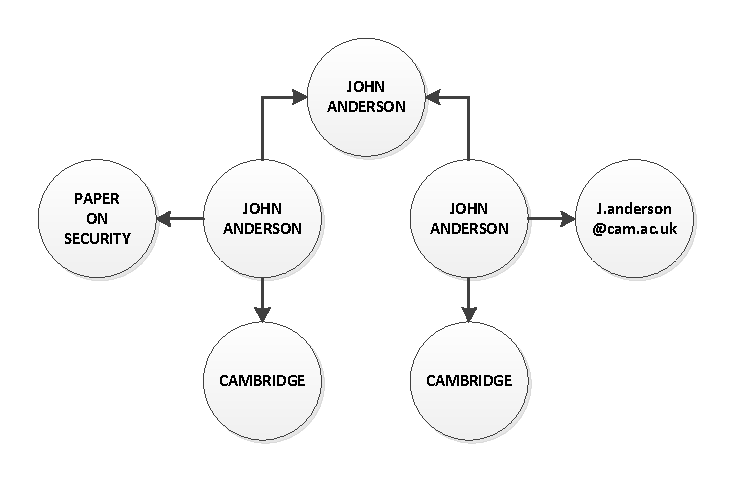
\includegraphics[width=0.6\textwidth]{fig/clusteringinstances}
	\caption{Grouping of instances under the same author}
	\label{fig:clusteringinstances}
\end{figure}

\subsection{Problem Domain}

As already said, our goal is to link different instances of an author. Therefore the properties of those instances have to be compared. In the case of the discovery of a new instance, it is infeasible to compare it with all the instances that were already found before. That would make the problem more and more complex over time. This forces us to narrow down the problem space. For a certain instance $I_i$, we want to minimize the compared instances that do not represent the same author as this instance ("real" instances), while still trying to compare all instances that are real ones. This is formulated in equation \autoref{eq:problemspace}.

\begin{equation}
\min |I^\text{compared}_i\backslash I^\text{real}_i|,\ s.t.\ I^\text{real}_i \subseteq I^\text{compared}_i \subseteq I
\label{eq:problemspace}
\end{equation}

Names are still an important property for person identification. If we find two totally different names, we can say with confidence that they are not the same person. We let the case where the person in question would have undergone a namechange slip, this rare incident would lead us too far. Additionaly, people almost always refer to people by using their name. When information is found, we can be almost sure that it will be accompanied by a name. These properties make names an excellent candidate for narrowing down our problem space.

Note that in the example used in the previous section, we sidestepped an extra difficulty. It assumed that our source contained two instances associated with the same name. When people have totally different names, they are not the same. When they have the same name, they could be the same. But what about those names that are almost the same? If the names are not too different, the instances must certainly be compared. The definition of "too different" needs to comply with equation \autoref{eq:problemspace}.

Narrowing down the problem space using names is done using two rules. Two instance will never be compared if any of the following two conditions are satisfied:

\begin{enumerate}
\item Their family names are different.
\item The notation of their names is too different.
\end{enumerate}

The formal definition of a "family name" and the exact meaning of "too different" will be explained in more detail in .... REF. The structural represenation of name notations will be further explained in the next section.

\subsection{Name notations}

Concerning the structure of name notations in our model we have also walked two different paths. Again, we will first explain the most obvious one. 

\paragraph{Instance-Author} Every instance belongs to a certain author (due to clustering), but it also has a number of authors it could belong to. These authors are called match-authors. If similar instances are found that are part of a match-author, it would be possible for an instance to become part of this author as well (reclustering). The problem with this approach is that an author is completely defined by its instances which change over time. The decision if an author should be a match-author therefore changes along. The problem is illustrated in \autoref{fig:namematchproblem}. Information on J. and Jake Anderson has lead us to the conclusion that they are probably the same person, the instances are clustered. Before, it was considered possible that instance John Anderson belonged to the author J. Anderson. Because of earlier clustering, J. Anderson is now actually Jake Anderson. It comprises information of both J. and Jake Anderson. This means that John Anderson will also be compared to the instance with Jake Anderson. If we would re-match John Anderson, it would never have been considered to be a part of Jake Anderson (different names). This is an inconsistency.

\begin{figure}[htbp]
	\centering
		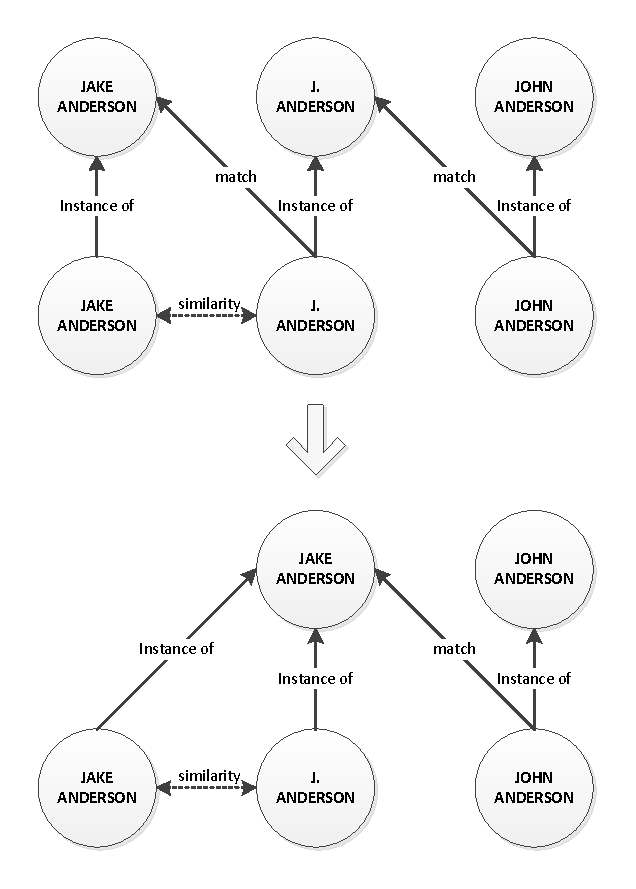
\includegraphics[width=0.6\textwidth]{fig/namematchproblem}
	\caption{Problem with instance-author matching}
	\label{fig:namematchproblem}
\end{figure}

\paragraph{Name-Name} It is better practice to keep authors and names more isolated. This new approach is illustrated in \autoref{fig:namematchsolution}. In this situation, instances associated with the name Jake Anderson will never be compared with instances with name John Anderson.

\begin{figure}[htbp]
	\centering
		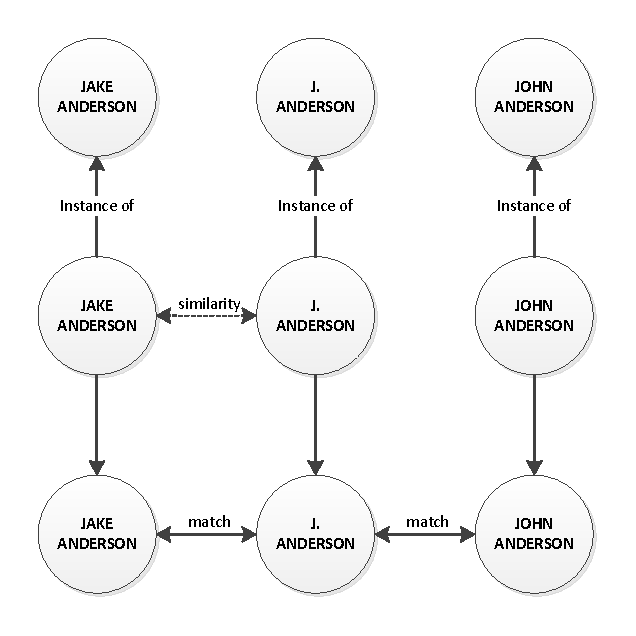
\includegraphics[width=0.6\textwidth]{fig/namematchsolution}
	\caption{Solution of instance-author matching: pure name matching}
	\label{fig:namematchsolution}
\end{figure}

\subsection{Conclusion and Overview}

We have addressed all the main issues that arose during the design of a structure that can stisfy the efficiency and flexibility needed according to the foundation acknowledgements (REF). We will finish with a final example of the typical structure of the graph as a theorethical model. This overview can be found in \autoref{fig:graphstructureoverview}.

\begin{figure}[htbp]
	\centering
		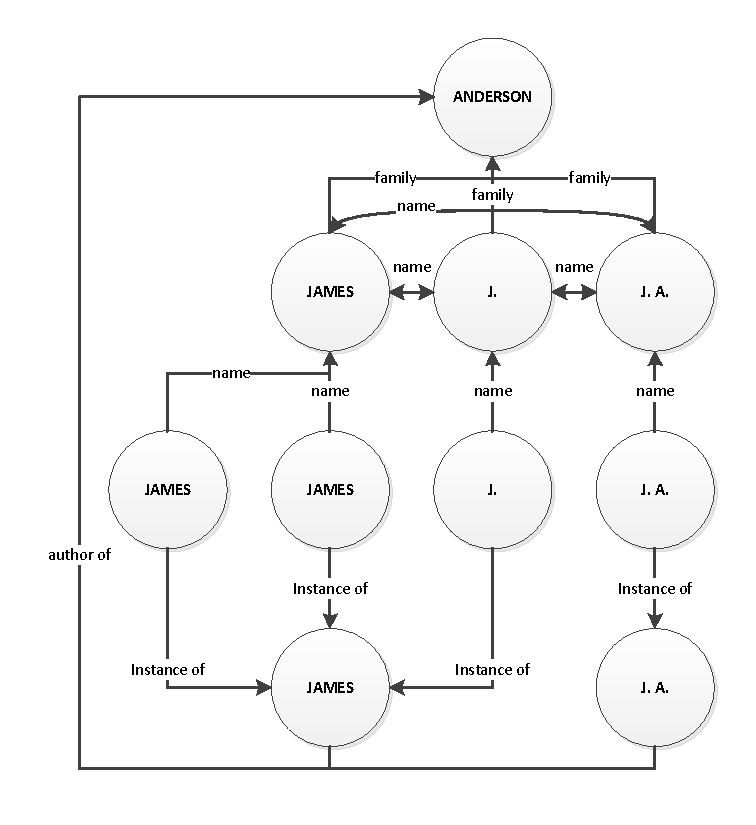
\includegraphics[width=0.75\textwidth]{fig/graphstructureoverview}
	\caption{Overview of the structure layer of the graph model}
	\label{fig:graphstructureoverview}
\end{figure}

\section{Three layer model: information layer}

% TODO

\section{Three layer model: similarity layer}

As we have stated several times, the goal is to link instances together to form an author. Until now, linking was just an action of an algorithm. If an algorithm decides that two instances represent the same author, the algorithm links them together (by actually changing the "instance of" edges in the graph). But what about the links itself? Should these links also represent a "physical" concept in our model? This is a question answered by the similarity layer.

\paragraph{Weighted Similarities} When two instances are compared, we need to compare their properties. Properties could be email addresses, locations, people we work with, \ldots When compared instances have the location "Belgium" in common, but their email addresses are different, it would be doubtful that these two are the same. In the opposite situation (the same email address and a different location) it would be alot more probable for these instances to represent the same person. We can conclude that some properties are more distinctive than others. When the value of two properties is (partially) the same (degree of equality), we speak of a similarity. These similarities are assigned a normalized weight proportional to the distinctiveness of the property and the degree of equality.
% misschien ook nog een formele definitie hier

\paragraph{Stateful Similarities} There is a reasons why similarities have to actually be persisted. According to the foundation acknowledgements [REF] we are in need of a constantly changing output. This means that the system will incrementally build towards a solution. If we only want to calculate as few as necessary similarities when new information is found, all other similarities must already be present. With the similarity layer (plane) enabled, \autoref{fig:graphstructureoverview} could become \autoref{fig:graphstructureoverviewsim} (We left out the family node).

\begin{figure}[htbp]
	\centering
		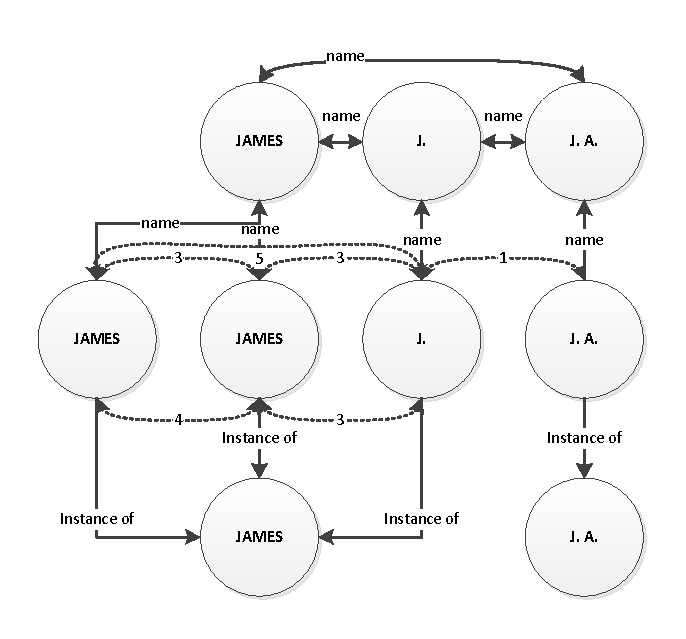
\includegraphics[width=0.75\textwidth]{fig/graphstructureoverviewsim}
	\caption{Overview of the structure layer of the graph model with the similarity layer}
	\label{fig:graphstructureoverviewsim}
\end{figure}

\section{Rules}

%introductie

%3 scopes: umbrella: matched instances
%- matching-name instances
%- equal-name instances
%- shared-cluster instances

\begin{mydef}
\label{def:rule}
A \textbf{Rule} is a mechanism that issues a complex query on the graph-model in order to find similarities between instances.
\end{mydef}

\subsection{Community Rule}

Authors often work together with the same people, writing multiple publications together. Instances that are linked (due to co-authoring) to instances belonging to the same author or with a similar name are more similar themselves because of these links. This is a property that will be exploited by the community rule. We can distinguish several situations, some yielding a stronger similarity than others. We list them below ordered by increasing similarity, each of them is illustrated with an example.

Before going through each situation, let us sketch the common situation. There exists an instance X with a matched instance Y

\paragraph{Name Equality} 

\paragraph{Name Matching}

\paragraph{Shared Cluster}

\begin{figure}[htbp]
	\centering
		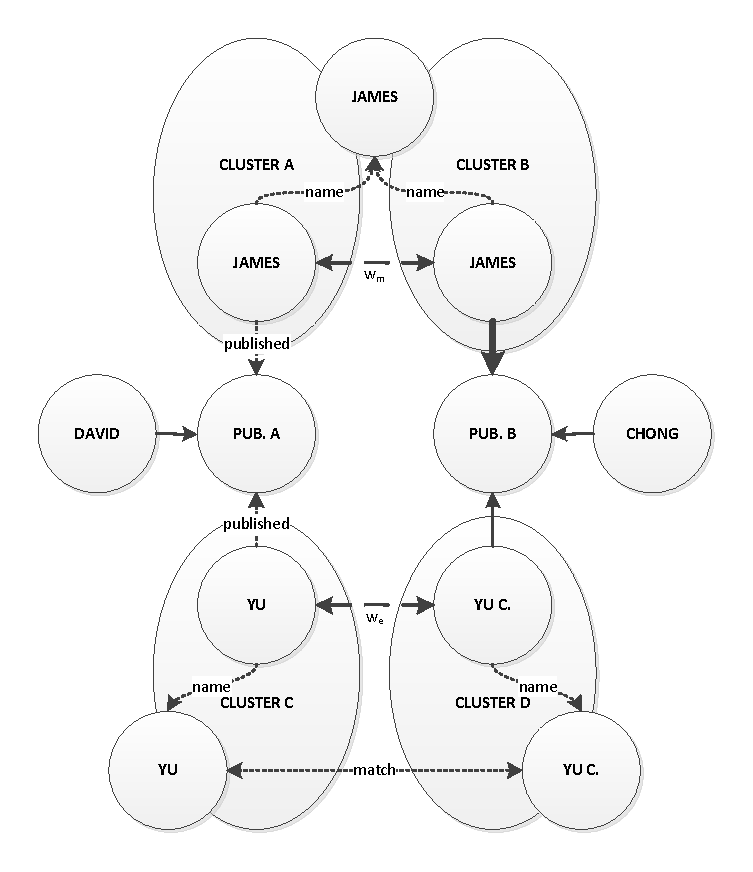
\includegraphics[width=0.75\textwidth]{fig/coauthorrulenameeq}
	\caption{}
	\label{fig:coauthorrulenameeq}
\end{figure}

\begin{figure}[htbp]
	\centering
		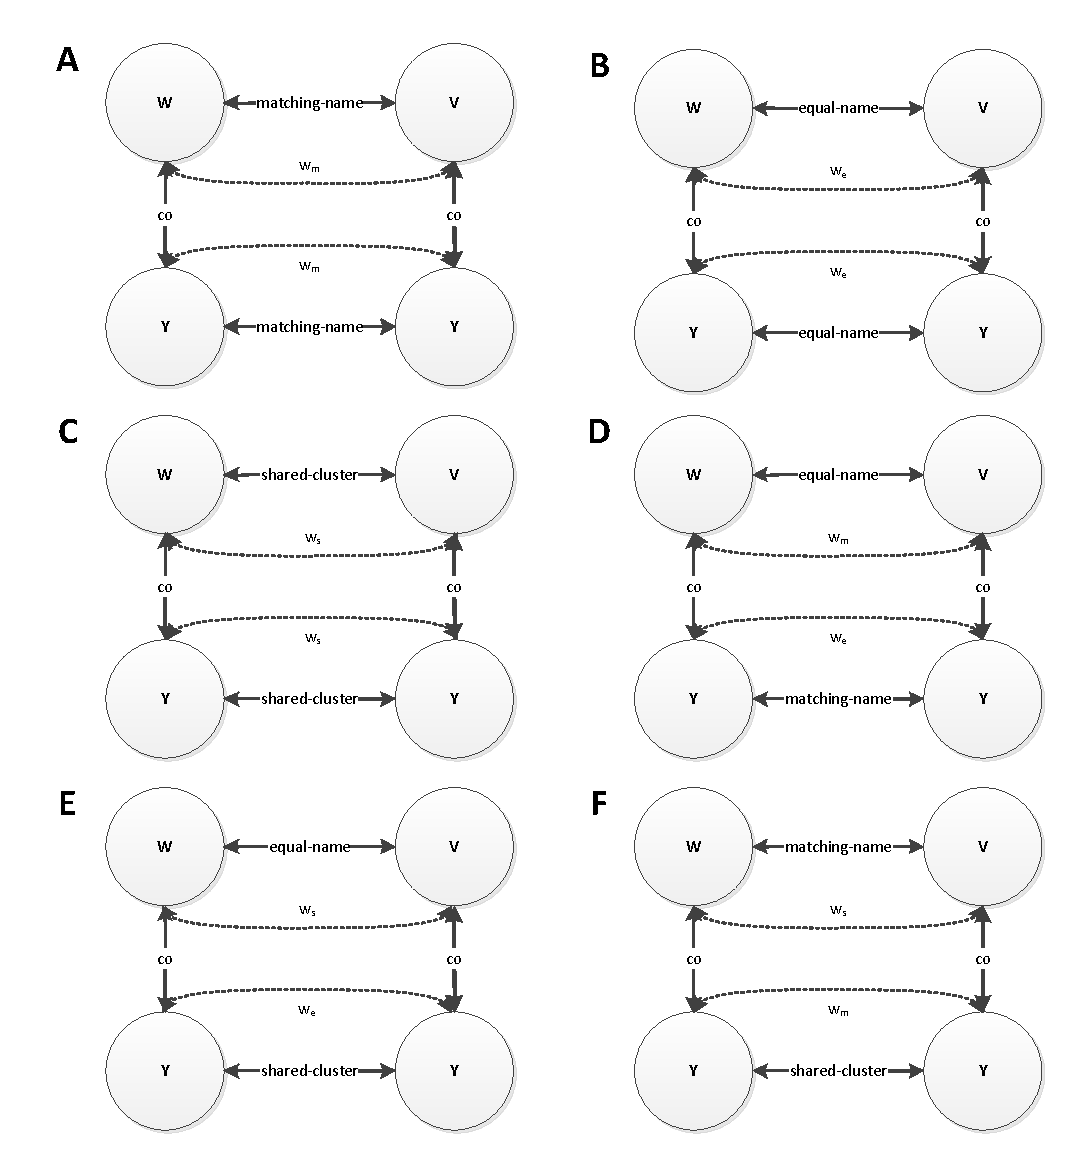
\includegraphics[width=0.9\textwidth]{fig/coauthorrulecases}
	\caption{}
	\label{fig:coauthorrulecases}
\end{figure}

\subsection{Interest Rule}

\subsection{Email Rule}

\subsection{Affiliation Rule}